% Реберная раскраска кубического графа для устранения конфликтов при проведении вычислений на неструктурированной поверхностной расчетной сетке.
\subsection{Реберная раскраска дуального графа \\ поверхностной неструктурированной \\ расчетной сетки в 3 цвета}

Будем рассматривать проблему распараллеливания вычислений на общей памяти применительно к задаче расчета обледенения поверхности с помощью конечно-объемного метода \cite{Gulicheva2024}.
Моделирование процесса обледенения поверхности тела выполняется итерационно.
На каждой итерации расчетов в каждой расчетной ячейке производится решение системы уравнений массового и теплового балансов, из которой получаются основные данные состояния расчетной ячейки (температура, количество жидкой воды и накопленного льда и другие).
Между расчетными итерациями выполняется расчет протекания потоков жидкости между соседними ячейками (потоки массы и тепла через границы ячеек).
Также в зависимости от настроек решателя через заданные промежутки времени выполняется пересчет геометрии поверхности тела за счет накопленной в ее ячейках массы льда.
Расчеты обледенения выполняются на неструктурированной поверхностной расчетной сетке с треугольными ячейками.

\begin{lstlisting}[caption={Расчет протекания потоков через ребро сетки.}, label={lst:text_3_flows_through_edge}]
void Edge::calc_flows()
{
    // cells pair
    Cell* fst = ...;
    Cell* sec = ...;

    // flows calculation
    double flow_w = ...;
    double flow_q = ...;

    // flows correction
    fst->flow_out_w += flow_w;
    fst->flow_out_q += flow_q;
    sec->flow_out_w -= flow_w;
    sec->flow_out_q -= flow_q;
}
\end{lstlisting}

Пересчет состояния ячейки выполняется независимо от других ячеек, данные вычисления могут выполняться параллельно.
Пересчет потоков массы и тепла выполняются через каждое ребро расчетной сетки, при этом поток перетекает из одной инцидентной ребру ячейки в другую.
Общая схема пересчета потоков для одного ребра может выглядеть так, как представлено на листинге~\ref{lst:text_3_flows_through_edge}.

Для выполнения пересчета потоков для всех ребер домена\label{term:domain5} расчетной сетки необходимо обработать все ребра в цикле (см. листинг~\ref{lst:text_3_flows_through_edges}).

\begin{lstlisting}[caption={Расчет протекания потоков для всех ребер домена.}, label={lst:text_3_flows_through_edges}]
for (auto e : own_edges)
{
    e->calc_flows();
}
\end{lstlisting}

При обработке ребер домена расчетной сетки в цикле возникает желание распараллелить или векторизовать этот цикл.
При распараллеливании вычислений с помощью OpenMP\label{abbr:openmp2} следует учитывать конфликты по данным, которые могут возникнуть при выполнении корректировки потоков (в случае если несколько потоков начнут одновременно изменять значение одной области памяти).
Для устранения этих конфликтов достаточно выполнять операции корректировки потоков в атомарном режиме, как показано на листинге~\ref{lst:text_3_atomic_flows}.

\begin{lstlisting}[caption={Атомарные операции корректировки потоков.}, label={lst:text_3_atomic_flows}]
#pragma omp atomic
fst->flow_out_w += flow_w;
#pragma omp atomic
fst->flow_out_q += flow_q;
#pragma omp atomic
sec->flow_out_w -= flow_w;
#pragma omp atomic
sec->flow_out_q -= flow_q;
\end{lstlisting}

Использование \texttt{\#pragma omp atomic} гарантирует, что указанная команда одновременно будет обрабатываться только одним потоком (то есть, что между чтением старого значения переменной и записью нового значения не попадут операции другого потока).
При большом количестве используемых потоков это может приводить к потерям производительности.
Следует отдельно отметить, что такой подход не сработает при попытке векторизации\label{term:vectorization} рассматриваемого цикла.
Зачастую вычисление самих потоков через ребро не содержит сложного управления, и может быть легко векторизовано, но векторизации всего цикла мешают зависимости по данным при корректировке потоков.
В рассматриваемом случае можно избавиться от зависимости по данным путем разбиения исходного множества ребер сетки на такие подмножества, чтобы параллельная обработка ребер каждого отдельного подмножества не приводила к возникновению конфликтов при корректировке потоков.

\subsubsection{Сведение задачи распараллеливания вычислений \\ к реберной раскраске}

Будем решать задачу разрешения конфликтов между ребрами расчетной сетки с помощью реберной раскраски графа конфликтов.
Такой подход является достаточно естественным \cite{Gilfanov2021Coloring}, и в нашем случае вершины графа конфликтов будут иметь низкую степень, что свидетельствует о допустимости реберной раскраски в небольшое количество цветов.

Рассмотрим ситуацию, при которой возможно возникновение конфликта при корректировке потоков во время параллельной обработки двух ребер расчетной сетки.
Такой конфликт возможен в том случае, когда оба обрабатываемых ребра являются инцидентными одной и той же ячейке.
Рассмотрим дуальный граф\label{term:dual_graph3} нашей расчетной сетки -- то есть граф, вершины которого соответствуют ячейкам расчетной сетки, а ребро проведено между двумя вершинами в том и только том случае, когда две соответствующие ячейки расчетной сетки являются соседними по ребру.
Без ограничения общности будем считать, что рассматриваемая расчетная сетка не имеет краев, то есть каждая ее ячейка имеет ровно трех соседей.
В этом случае ее дуальный граф будет кубическим.
При этом задача разбиения ребер расчетной сетки на неконфликтующие множества сводится к построению реберной раскраски дуального графа.
В процессе нахождения реберной раскраски построенного дуального графа зададимся вопросом, вызывающим  исследовательский интерес -- в какое минимальное количество цветов можно раскрасить этот граф.
При этом будем считать, что мы рассматриваем только односвязные поверхности.
Таким образом, анализируемых дуальный граф является плоским кубическим графом.
Также отметим, ни одна расчетная ячейка исходной сетки не может быть соседней себе самой, а значит в построенном дуальном графе нет мостов.
То есть объектом нашего исследования является плоский кубический граф без мостов.

Алгоритмы раскраски плоского кубического графа без мостов в 5 и 4 цветов являются достаточно тривиальными и описаны в лемме~\ref{lem:text_3_graph_prim_coloring5} и лемме~\ref{lem:text_3_graph_prim_coloring4}.
Также в разделе~\ref{sec:text_3_graph_prim} было отмечено возможность раскраски такого графа в 3 цвета.
Если кубический граф допускает правильную реберную раскраску в 3 цвета, то такая раскраска называется раскраской Тейта\label{term:coloring_tait}.
В цикле работ \cite{Kurapov2018,Kurapov2020,Kurapov2020Mono} авторы предлагают способ построения раскраски Тейта для плоских кубических графов, который мы будем использовать в этом разделе.
Кубический граф, порожденный односвязной поверхностной расчетной сеткой, является плоским и не содержит мостов, поэтому такой способ построения раскраски Тейта для него применим.

\subsubsection{Редуцирование кубического графа по ребру \\ и его восстановление}

Рассмотрим принцип и реализацию алгоритма построения раскраски Тейта для кубического графа, являющегося дуальным графом для замкнутой поверхностной неструктурированной расчетной сетки.
В работах \cite{Kurapov2018,Kurapov2020} рассматривается подход к построению раскраски Тейта путем удаления ребер из исходного плоского кубического графа.
Ребра удаляются по тех пор, пока не будет получен кубический граф с уже известной раскраской.
После этого ребра возвращаются в граф в обратном порядке с соответствующей коррекцией раскраски.
Операцию удаления ребра из графа будем называть редуцированием кубического графа по ребру.
Для того чтобы редуцирование кубического графа по ребру можно было использовать для построения раскраски Тейта, необходимо уметь провести последовательность редукций до достижения простого по структуре кубического графа, раскраска которого не представляет сложности.
При этом, в получающихся графах допустимо наличие параллельных ребер, однако запрещено появление петель, так как раскраска Тейта для кубического графа с петлями невозможна.
Рассмотрим операцию редуцирования графа более подробно.

Сначала рассмотрим выполнение редуцирования кубического графа по ребру $e$ с концами $v_1$ и $v_2$, где инцидентными ребрами вершины v1 являются ребра $e$, $e_1(v_1)$, $e_2(v_1)$, а инцидентными ребрами вершины $v_2$ являются ребра $e$, $e_1(v_2)$, $e_2(v_2)$, а также среди ребер $e$, $e_1(v_1)$, $e_2(v_1)$, $e_1(v_2)$, $e_2(v_2)$ нет параллельных (см. рис.~\ref{fig:text_3_edge_coloring_1}, слева).
Из этого следует, что существует только одно ребро, соединяющее вершины $v_1$ и $v_2$.
В этом случае будем говорить, что редуцирование выполняется по уникальному ребру $e$.

\begin{figure}[ht]
\centering
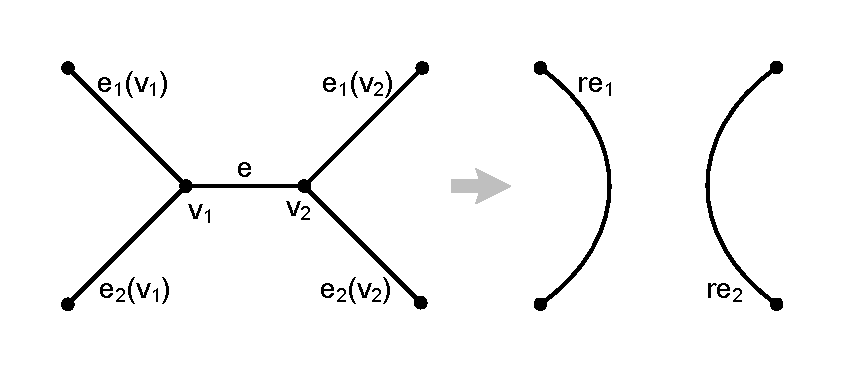
\includegraphics[width=0.8\textwidth]{./pics/text_3_edge_coloring/1-pic-reduce-edge-type-1.pdf}
\singlespacing
\captionstyle{center}\caption{Редуцирование по уникальному ребру.}
\label{fig:text_3_edge_coloring_1}
\end{figure}

При выполнении редуцирования по ребру $e$ само ребро $e$ удаляется, также удаляются вершины $v_1$ и $v_2$, ребра $e_1(v_1)$ и $e_2(v_1)$ склеиваются в результирующее ребро $re_1$, ребра $e_1(v_2)$ и $e_2(v_2)$ склеиваются в ребро $re_2$ (см. рис.~\ref{fig:text_3_edge_coloring_1}, справа).

Другим случаем редуцирования является вариант, при котором также концами рассматриваемого ребра $e$ являются вершины $v_1$ и $v_2$, однако между ними проходит еще одно ребро, без ограничения общности будем считать, что это ребро $e_2(v_1) = e_2(v_2)$ (см. рис.~\ref{fig:text_3_edge_coloring_2}, слева).
В этом случае при редуцировании удаляется ребро $e$, удаляются вершины $v_1$ и $v_2$, а все три ребра $e_1(v_1)$, $e_2(v_1) = e_2(v_2)$, $e_1(v_2)$ склеиваются в единое ребро $re_1 = re_2$ (см. рис.~\ref{fig:text_3_edge_coloring_2}, справа).
Такой шаг редуцирования будем называть редуцированием по параллельному ребру.

\begin{figure}[ht]
\centering
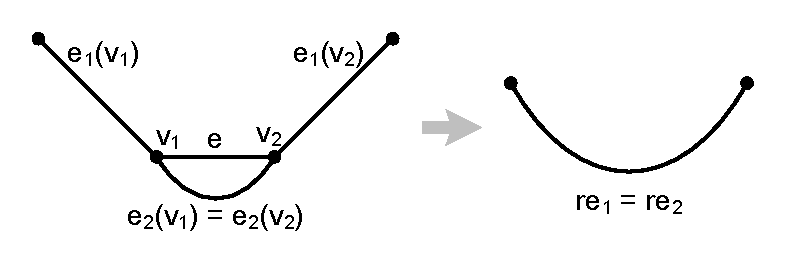
\includegraphics[width=0.8\textwidth]{./pics/text_3_edge_coloring/2-pic-reduce-edge-type-2.pdf}
\singlespacing
\captionstyle{center}\caption{Редуцирование по параллельному ребру.}
\label{fig:text_3_edge_coloring_2}
\end{figure}

Отдельно отметим случай, когда между двумя вершинами проходит три параллельных ребра.
Если мы достигли такого графа, то это и есть минимальный кубический граф, построение раскраски для которого очевидно, и от которого нужно двигаться в обратную сторону, постепенно восстанавливая исходный граф.
Также следует рассмотреть случай, при котором после редуцирования по уникальному ребру граф перестает быть связным.
Это значит, что в исходном графе ребро $e$ было мостом, такие графы рассматривать не будем.
В других случаях в графе найдется либо уникальное, либо параллельное ребро, по которому можно осуществить следующий шаг редуцирования.

В качестве примера рассмотрим редуцирование графа, представляющего собой куб, как показано на рис.~\ref{fig:text_3_edge_coloring_3}.

\begin{figure}[ht]
\centering
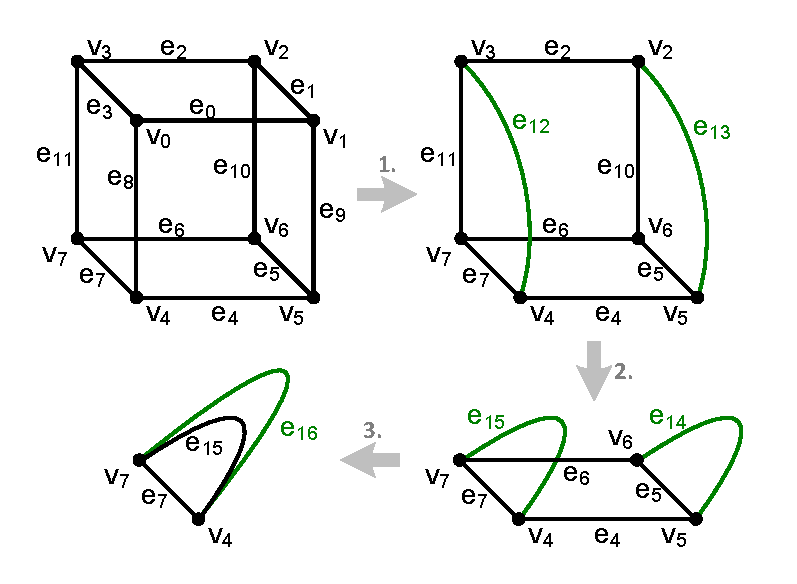
\includegraphics[width=0.8\textwidth]{./pics/text_3_edge_coloring/3-reduce-0.pdf}
\singlespacing
\captionstyle{center}\caption{Полное редуцирование графа.}
\label{fig:text_3_edge_coloring_3}
\end{figure}

На рис.~\ref{fig:text_3_edge_coloring_3} представлен кубический граф, содержащий 8 вершин $v_0$ -- $v_7$ и 12 ребер $e_0$ -- $e_{11}$.
Будем считать, что нижние индексы в именах вершин и ребер являются также их идентификаторами.
Для полного редуцирования указанного графа требуется выполнение 3 шагов, которые могут быть записаны в историю редуцирования следующим образом:

$e_0 [(v_0 : e_3, e_8 \rightarrow e_{12}), (v_1 : e_1, e_9 \rightarrow e_{13})]$

$e_2 [(v_2 : e_{13}, e_{10} \rightarrow e_{14}), (v_3 : e_{12}, e_{11} \rightarrow e_{15})]$

$e_5 [(v_5 : e_4, e_{14} \rightarrow e_{16}), (v_6 : e_6, e_{14} \rightarrow e_{16})]$

По такой записи истории редуцирования можно идентифицировать каждый шаг, определить его тип (редуцирование по уникальному ребру или по параллельному) и выполнить восстановление графа.

Опираясь на указанные операции редуцирования можно описать алгоритм построения раскраски Тейта во время восстановления графа.

\subsubsection{Алгоритм реберной раскраски кубического графа в 3 цвета}

Прежде чем перейти к описанию алгоритма построения раскраски, рассмотрим центральный объект, который будет использован в этом построении.
Без ограничения общности будем считать, что раскраска выполняется в следующие цвета: красный, синий и зеленый, -- эти же цвета будем приводить на иллюстрациях.
Путь ребра некоторого кубического графа правильным образом раскрашены в три цвета.
Рассмотрим произвольные два цвета -- например, красный и синий.
Если рассмотреть все ребра, покрашенные в эти два цвета, а также все инцидентные им вершины, то получим граф порядка 2, у которого в каждой вершине сходятся разноцветные ребра.
Очевидно, такой граф является объединением простых циклов четной длины (двухцветных циклов)\label{term:bicolor_cycle}.
На рис.~\ref{fig:text_3_edge_coloring_4} приведен пример такого двухцветного красно-синего цикла.

\begin{figure}[ht]
\centering
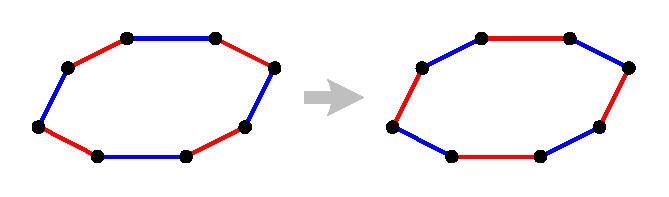
\includegraphics[width=0.6\textwidth]{./pics/text_3_edge_coloring/4-bicolor-cycle.pdf}
\singlespacing
\captionstyle{center}\caption{Полная замена цветов в двухцветном цикле.}
\label{fig:text_3_edge_coloring_4}
\end{figure}

С таким двухцветным циклом можно выполнять следующие операции.
Во-первых, для всех ребер двухцветного цикла можно заменить цвет на противоположный, после чего раскраска в исходном графе останется правильной (см. рис.~\ref{fig:text_3_edge_coloring_4}).
Также можно применить перекраску в противоположный цвет не всех ребер цикла, а только расположенных между двумя фиксированными ребрами $e_1$ и $e_2$ (на рис.~\ref{fig:text_3_edge_coloring_5} приведены два варианта такой перекраски в порядке обхода цикла по часовой и против часовой стрелки).
При такой перекраске ребер в цикле возникает два конфликта по цветам: между ребрами $e_1$ и $e_2$ и их перекрашенными соседями.

\begin{figure}[ht]
\centering
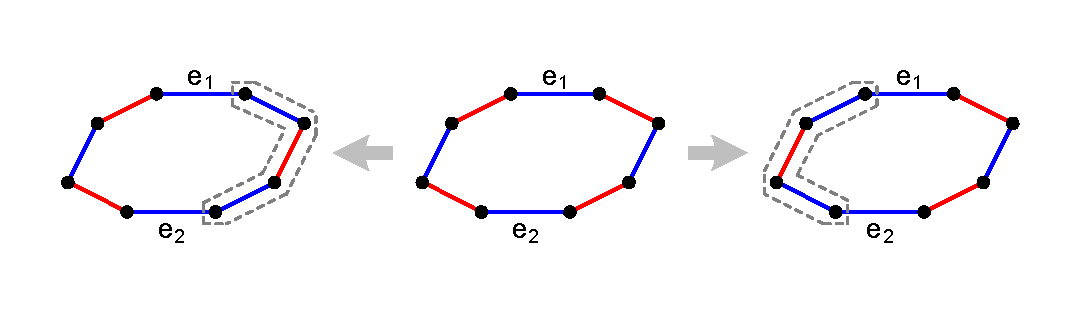
\includegraphics[width=0.8\textwidth]{./pics/text_3_edge_coloring/5-bicolor-cycle-partial-switch.pdf}
\singlespacing
\captionstyle{center}\caption{Частичная замена цветов в двухцветном цикле.}
\label{fig:text_3_edge_coloring_5}
\end{figure}

Смысл частичной замены цветов в двухцветном цикле становится понятным, если возникает необходимость поместить в граф новое ребро.
На рис.~\ref{fig:text_3_edge_coloring_6} продемонстрирована операция, при которой выполняется частичная перекраска цикла между ребрами $e_1$ и $e_2$, а затем на ребра $e_1$ и $e_2$ добавляются новые вершины $v_1$ и $v_2$ соответственно, между которыми проводится ребро.
В завершение полученные после разбиения ребер $e_1$ и $e_2$ более мелкие ребра перекрашиваются для устранения конфликтов.
Новое проведенное ребро при этом перекрашивается в третий свободный цвет, что приводит к сохранению правильной раскраски во всем графе.
Таким образом, выбрав два произвольных ребра на любом двухцветном цикле, мы можем добавить новое ребро с концами на выбранных ребрах, а затем перекрасить ребра и сохранить правильную реберную раскраску.
Такую операцию будем называть восстановлением ребра по двухцветному циклу.

\begin{figure}[ht]
\centering
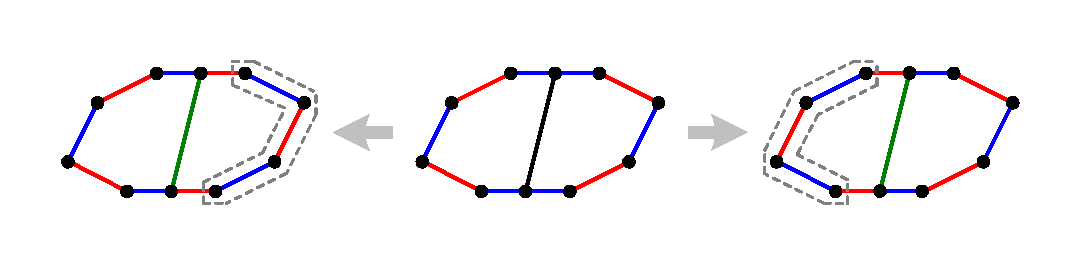
\includegraphics[width=0.8\textwidth]{./pics/text_3_edge_coloring/6-bicolor-cycle-new-edge.pdf}
\singlespacing
\captionstyle{center}\caption{Замена цветов в двухцветном цикле при добавлении нового ребра.}
\label{fig:text_3_edge_coloring_6}
\end{figure}

Также нам понадобится операция поиска двухцветного цикла, начиная с произвольного ребра $e$, и содержащего ребра цветов $\gamma(e)$ и $c \ne \gamma(e)$. Такой цикл всегда существует и он ровно один.

Теперь, имея в своем распоряжении три простые операции: поиск двухцветного цикла по ребру и второму цвету, перекраска двухцветного цикла и восстановление ребра по двухцветному циклу, -- мы можем описать алгоритм восстановления одного шага редуцирования графа с сохранением правильной реберной раскраски (см. рис.~\ref{fig:text_3_edge_coloring_7}).

Дополнительно отметим, что восстановление шага редуцирования графа по параллельному ребру не представляет сложности, так как это локальная операция, которая затрагивает единственное результирующее ребро. Поэтому рассмотрим подробно только восстановление шага редуцирования по уникальному ребру.

Пусть мы имеем шаг редуцирования графа, результирующими ребрами после выполнения которого являются различные ребра $re_1$ и $re_2$.
В процессе восстановления мы должны поместить на эти ребра новые вершины $v_1$ и $v_2$ соответственно, провести между ними ребро и выполнить коррекцию раскраски.
Опишем последовательность действий в этом случае.

Вариант 1. Если результирующие ребра $re_1$ и $re_2$ имеют разные цвета, то найдем двухцветный цикл, начиная с ребра $re_1$, включающий в себя ребра цветов $\gamma(re_1)$ и $\gamma(re_2)$.
Если найденный цикл содержит также и ребро $re_2$, то можно выполнить восстановление исходного ребра по найденному двухцветному циклу.
В противном случае перекрасим найденный двухцветный цикл.
Так как перекрашивание затронет только ребро $re_1$, то после этой операции мы получим ситуацию, в которой ребра $re_1$ и $re_2$ имеют один цвет. В этом случае переходим ко второму варианту.

\begin{figure}[ht]
\centering
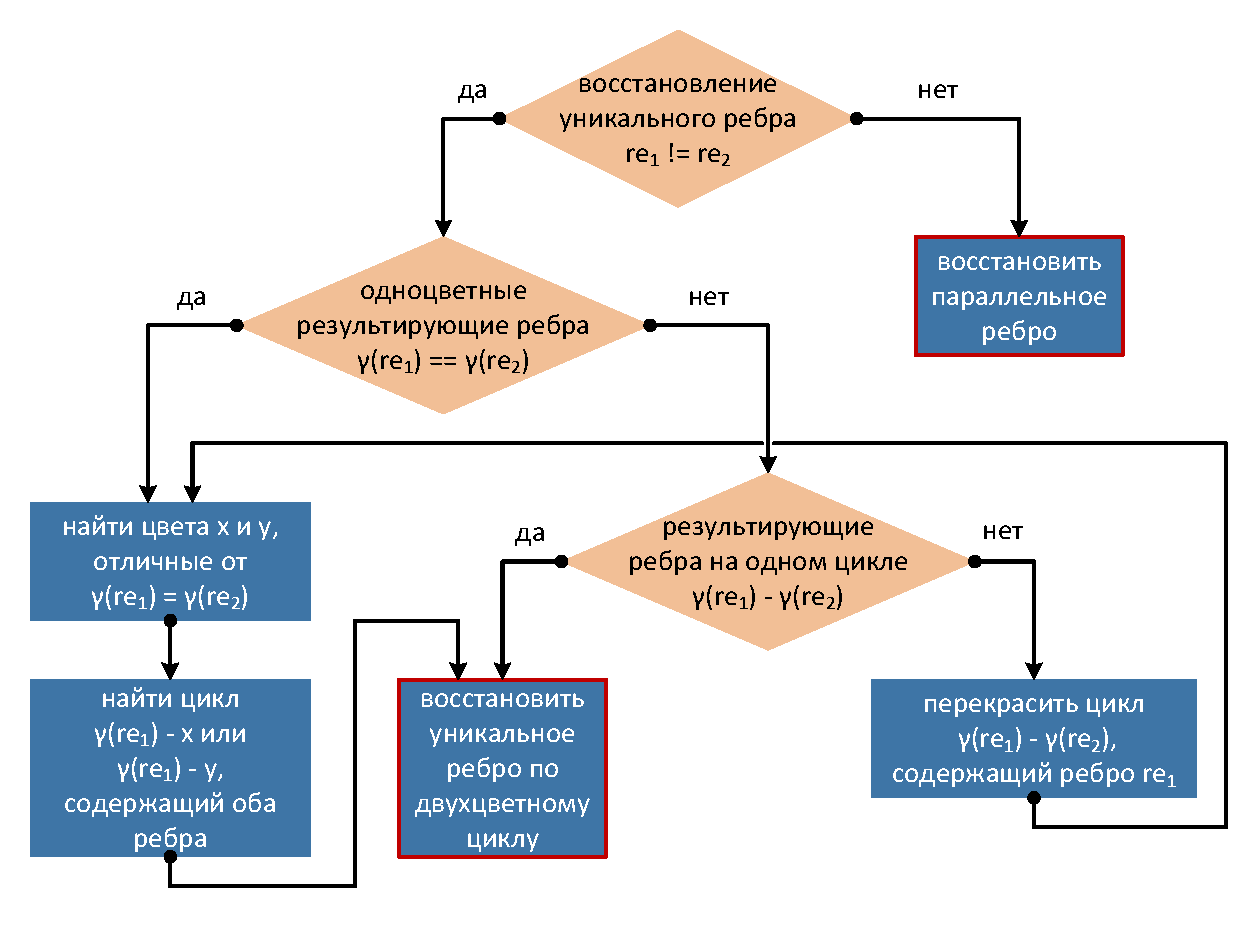
\includegraphics[width=1.0\textwidth]{./pics/text_3_edge_coloring/7-algorithm.pdf}
\singlespacing
\captionstyle{center}\caption{Итерация алгоритма восстановления и перекраски графа.}
\label{fig:text_3_edge_coloring_7}
\end{figure}

Вариант 2. Если результирующие ребра $re_1$ и $re_2$ имеют один и тот же цвет, то рассмотрим два оставшихся цвета: $x$ и $y$.
Рассмотрим два двухцветных цикла, начиная с ребра $re_1$.
Причем в первый цикл будем включать ребра с цветами $\gamma(re_1)$ и $x$, а во второй цикл будем включать ребра с цветами $\gamma(re_1)$ и $y$.
Если один из найденных двухцветных циклов будет содержать также и ребро $re_2$, то по этому циклу и нужно выполнить восстановление исходного ребра, которое было удалено из графа при редуцировании.
Вопрос содержания ребра $re_2$ в одном из двухцветных циклов $\gamma(re_1) - x$ и $\gamma(re_1) - y$ оставим без доказательства (его можно найти в \cite{Kurapov2018}).

\begin{figure}[ht]
\centering
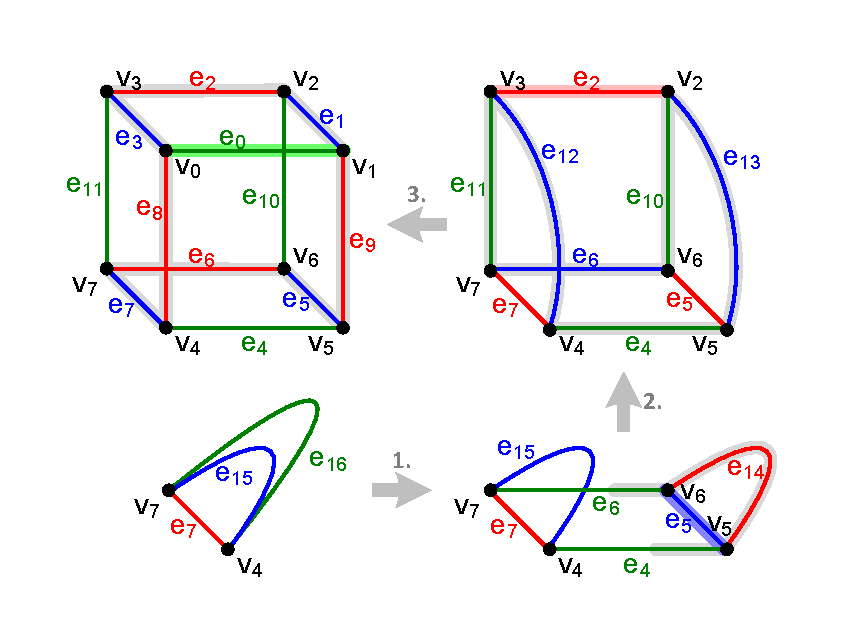
\includegraphics[width=0.8\textwidth]{./pics/text_3_edge_coloring/8-restore-and-repaint.pdf}
\singlespacing
\captionstyle{center}\caption{Восстановление и раскраска графа.}
\label{fig:text_3_edge_coloring_8}
\end{figure}

На рис.~\ref{fig:text_3_edge_coloring_8} приведена последовательность восстановления графа, редуцирование которого продемонстрировано на рис.~\ref{fig:text_3_edge_coloring_3}.
Приведем еще раз историю редуцирования графа:

$e_0 [(v_0 : e_3, e_8 \rightarrow e_{12}), (v_1 : e_1, e_9 \rightarrow e_{13})]$

$e_2 [(v_2 : e_{13}, e_{10} \rightarrow e_{14}), (v_3 : e_{12}, e_{11} \rightarrow e_{15})]$

$e_5 [(v_5 : e_4, e_{14} \rightarrow e_{16}), (v_6 : e_6, e_{14} \rightarrow e_{16})]$

Первый шаг восстановления относится к редуцированию по параллельному ребру.
Ребро $e_{16}$ разбивается на три ребра $e_6$, $e_{14}$, $e_4$ с помощью вершин $v_6$ и $v_5$.
Между вершинами $v_6$ и $v_5$ восстанавливается ребро $e_5$.
Ребра $e_6$ и $e_4$ наследуют зеленый цвет ребра $e_{16}$, а ребра $e_{14}$ и $e_5$ раскрашиваются в два оставшиеся цвета.

Второй шаг восстановления относится к редуцированию по уникальному ребру.
Сначала ищется красно-синий цикл, содержащий ребро $e_{14}$.
Так как он не содержит ребро $e_{15}$, то цикл из двух ребер $e_{14}-e_5$ перекрашивается.
После этого ищется сине-зеленый цикл, содержащий ребро $e_{14}$.
Это цикл $e_{14}-e_6-e_{15}-e_4$, и он содержит ребро $e_{15}$.
Происходит восстановление ребра по найденному двухцветному циклу.

Третий шаг восстановления также относится к редуцированию по уникальному ребру.
Так как существует сине-красный цикл $e_{12}-e_2-e_{13}-e_5-e_6-e_7$, то сразу можно выполнить восстановление ребра по этому циклу (а в этом случае можно выполнить восстановление и по сине-зеленому циклу, что приведет к другой раскраске).

Очевидно, что описанный алгоритм имеет квадратичную сложность по порядку графа, так как количество шагов восстановления пропорционально порядку исходного графа, а на каждом шаге восстановления уникального ребра необходимо выполнять поиск и перекраску двухцветных циклов, что в худшем случае пропорционально порядку текущего графа.

\subsubsection{Анализ полученных результатов}

Если мы рассматриваем кубический граф порядка $n$, то он содержит $\frac{3n}{2}$ ребер, причем $n$ четно.
Если данный граф допускает правильную реберную раскраску в 3 цвета, то в каждый из цветов раскрашено ровно $\frac{n}{2}$ ребер.
Таким образом, множество ребер распадается на 3 одинаковых по размеру подмножеств ребер без конфликтов.
Вызывает интерес вопрос о процентном соотношении ребер, раскрашенных в разные цвета, для жадной раскраски в 5 цветов при порядке графа, стремящемся к бесконечности.

\begin{figure}[ht]
\centering
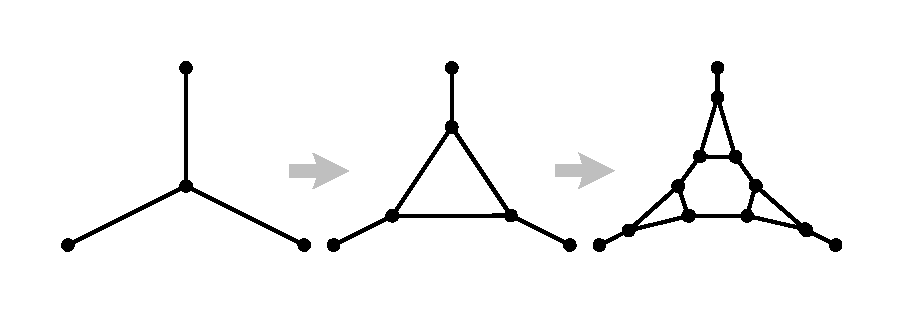
\includegraphics[width=0.8\textwidth]{./pics/text_3_edge_coloring/9-bubble.pdf}
\singlespacing
\captionstyle{center}\caption{Генерация кубического графа.}
\label{fig:text_3_edge_coloring_9}
\end{figure}

Для экспериментального получения такого распределения будем строить искусственные кубические графы следующим образом.
В качестве нулевого графа возьмем кубический граф $K_4$, далее последовательно в текущем кубическом графе будем случайным образом выбирать вершину и заменять ее на треугольную конструкцию, как показано на рис.~\ref{fig:text_3_edge_coloring_9}.
Вполне очевидно, что получающиеся таким образом графы будут кубические, и что они допускают правильную реберную раскраску в три цвета.
К полученным сгенерированным описанным способом кубическим графам порядка более $10^5$ был применен жадный линейный алгоритм реберной раскраски в 5 цветов.
Получившееся распределение цветов представлено на рис.~\ref{fig:text_3_edge_coloring_10}.

\begin{figure}[ht]
\centering
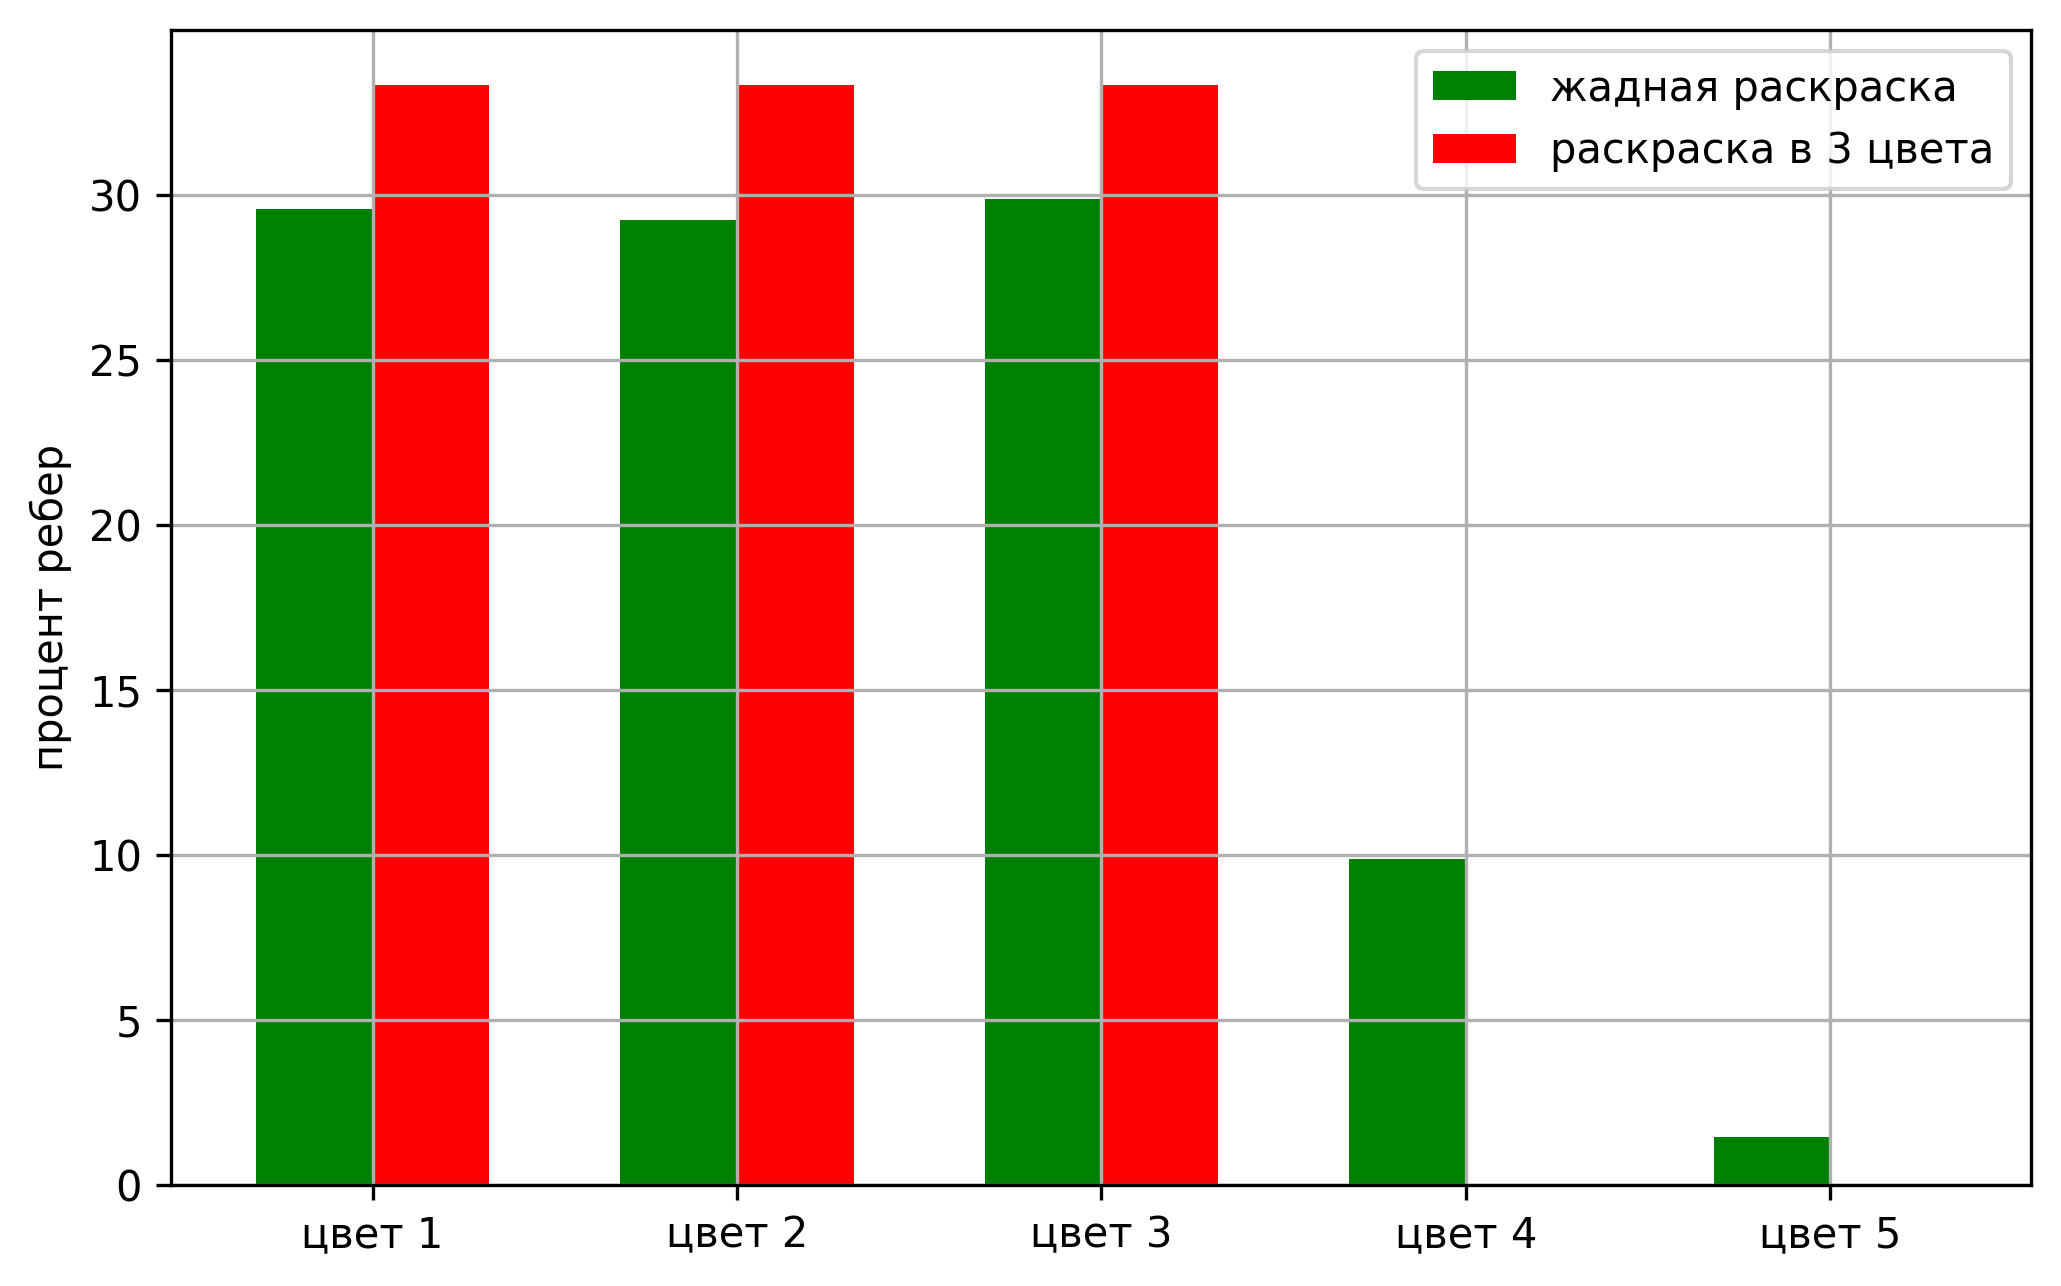
\includegraphics[width=0.6\textwidth]{./pics/text_3_edge_coloring/10-chart.png}
\singlespacing
\captionstyle{center}\caption{Распределение процентной доли цветов для разных раскрасок.}
\label{fig:text_3_edge_coloring_10}
\end{figure}

Из рис.~\ref{fig:text_3_edge_coloring_10} видно, что распределение цветов жадной раскраски устроено примерно следующим образом.
Большинство ребер кубического графа практически равномерно раскрасилось в 3 цвета, однако для окрашивания около 10\% ребер потребовалось использование четвертого цвета, а для окрашивания около 1,5\% ребер пришлось задействовать пятый цвет.

Для оценки целесообразности применения реберной раскраски для устранения конфликтов по данным при расчете потоков в задаче моделирования процесса обледенения поверхности были выполнены запуски модельной задачи на одном вычислительном узле на базе микропроцессора Intel Xeon Phi KNL\label{abbr:knl2} 7290.
Данный микропроцессор имеет 72 ядра, на каждом из которых может быть запущено до 4 потоков.
Таким образом, на этом микропроцессоре возможно распараллеливание запуска на 288 потоков.

Для сравнения эффективности методов устранения конфликтов при параллельном расчете потоков через границы ячеек замерялось ускорение вычислений при распараллеливании $s_{shr}$ эффективность распараллеливания $e_{shr}$.
Сравнивались два метода устранения конфликтов по доступу к данным: использование \texttt{omp atomic} операций и разделение множества ребер на неконфликтующие подмножества с помощью реберной раскраски.

\begin{figure}[ht]
\centering
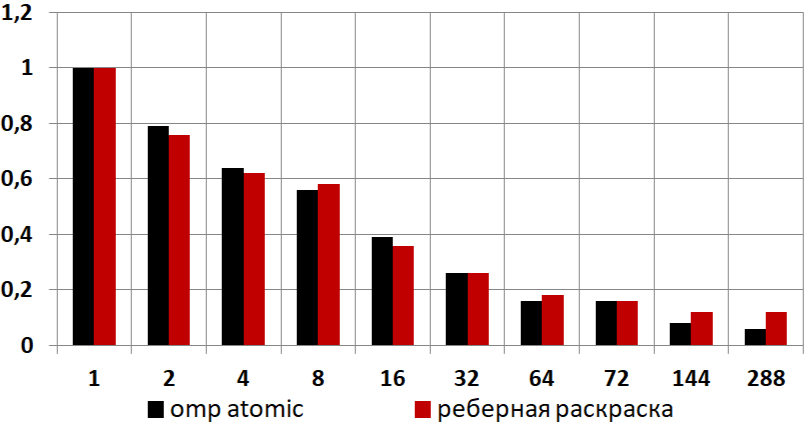
\includegraphics[width=1.0\textwidth]{./pics/text_3_edge_coloring/11-chart.png}
\singlespacing
\captionstyle{center}\caption{Эффективность распараллеливания пересчета потоков для разных способов устранения конфликтов по данным.}
\label{fig:text_3_edge_coloring_11}
\end{figure}

Из рис.~\ref{fig:text_3_edge_coloring_11} можно заметить, что при использовании распараллеливания на относительно небольшое количество потоков нет существенной разницы между описанными методами устранения конфликтов.
Однако при возрастании количества используемых потоков метод реберной раскраски становится гораздо эффективнее, чем использование директивы \texttt{omp atomic} с точки зрения эффективности распараллеливания.
